El papá de un estudiante del grado noveno ha comprado el maíz almacenado en un silo con forma de cilindro coronado por un cono invertido. El silo tiene un radio de 2 m; la parte cilíndrica tiene una altura de 10 m y la parte cónica (invertida) una altura de 3 m.

\begin{center}
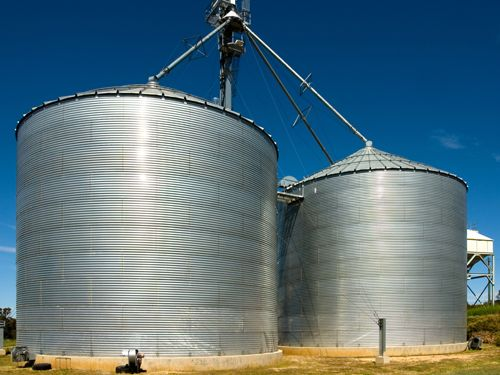
\includegraphics[width=0.4\linewidth]{res/image/silo_maiz.png}
\end{center}

El agricultor pagó aproximadamente \$18.000.000 por todo el contenido del silo y desea saber cuántos sacos de maíz de 25 kg puede obtener. Según información agrícola, un saco de maíz de 25 kg ocupa aproximadamente $0{,}03\ \text{m}^3$.

El comerciante que le vendió el maíz le asegura que del silo se pueden obtener cerca de 3.500 sacos, pero el agricultor desconfía de este valor y decide pedirle ayuda a su hijo, quien estudia en el colegio.

A partir de la información dada, determine si la cantidad de sacos indicada por el comerciante es razonable.

Explique su procedimiento, las decisiones tomadas y los conceptos geométricos utilizados. No se aceptan respuestas sin justificación.